\section{Introduction}\label{sec:introduction}

Rohde and Schramm formulated a square-lattice random-cluster interface
conjecture at the self-dual parameter for every fixed $0<q<4$
\cite[Conjecture~9.7 and the following discussion]{RohdeSchramm2005}.
They motivated the proposed relation between $q$ and the SLE parameter
using the dimensions of cluster perimeters predicted by Saleur and
Duplantier \cite{SaleurDuplantier1987}.  Schramm later restated the
problem in his collection of questions about conformally invariant
scaling limits \cite[Problem~2.6]{Schramm2006}.
We prove the predicted limit for every fixed $0<q<1$ in smooth
Jordan domains, with the finite wired/free law, lattice approximation,
and curve topology specified below. This gives the smooth-domain
formulation of the prediction; the concrete unit-square formulation of
Rohde and Schramm has a different boundary regularity. The argument
starts from the finite law at the self-dual parameter and does not
require prior identification of an infinite-volume critical point.

\subsection{The finite law and the main theorem}

Fix $q\in(0,1)$ and set
\begin{equation}\label{eq:parameters}
 d=\sqrt q=2\cos\lambda,
 \qquad p=\frac{d}{1+d},
 \qquad \rho=\frac{\lambda}{\pi},
 \qquad \kappa=\frac4{1-\rho}.
\end{equation}
Thus $\pi/3<\lambda<\pi/2$, $1/3<\rho<1/2$, and
$6<\kappa<8$. Let $D$ be a bounded Jordan domain with smooth simple
boundary, and let $a,b$ be distinct points on its boundary.
For each mesh $\delta$, let $D_\delta$ be the bounded interior of a
simple closed nearest-neighbor polygon in $\delta\Z^2$, and let
$a_\delta,b_\delta$ be distinct vertices of that polygon. Let
$G_\delta=(V_\delta,E_\delta)$ be the graph with vertex set
$V_\delta=\delta\Z^2\cap\overline{D_\delta}$ and edge set
$E_\delta$ consisting of all closed nearest-neighbor segments contained
in $\overline{D_\delta}$; write $E=E_\delta$.
Choose counterclockwise continuous parametrizations
$\beta_\delta:[0,1]\to\partial D_\delta$ and
$\beta:[0,1]\to\partial D$ that trace their boundaries once, satisfy
$\beta_\delta(0)=\beta_\delta(1)$ and $\beta(0)=\beta(1)$, and are
injective on $[0,1)$. Require
$\beta_\delta\to\beta$ uniformly. The cyclic parameters of
$a_\delta,b_\delta$ converge to the distinct cyclic parameters of
$a,b$. This initial approximation class excludes slit or pinched
polygon boundaries and marks in the interiors of lattice edges.

Choose one of the two closed boundary arcs from $a_\delta$ to $b_\delta$
as wired, including both endpoints. Identify all its vertices in the
component count and leave every other boundary vertex singleton.
For $A\subseteq E$, write $k_\xi(A)$ for the
number of components after that identification, including isolated
vertices. The random-cluster law is
\begin{equation}\label{eq:finite-target-law}
 \PP_{G_\delta}^{\xi}(A)
 =\frac{p^{|A|}(1-p)^{|E|-|A|}q^{k_\xi(A)}}
 {\sum_{B\subseteq E}p^{|B|}(1-p)^{|E|-|B|}q^{k_\xi(B)}}.
\end{equation}
For the interface drawing, declare exactly the boundary edges of the
wired arc open.
An open primal edge pairs adjacent medial half-edges around its dual
faces, and a closed primal edge pairs them around its primal endpoints.
The boundary turns between the primal wired arc and complementary dual
wired arc leave one distinguished strand. Denote by $\eta_\delta$ this
strand oriented from the medial endpoint associated with $a_\delta$ to
the endpoint associated with $b_\delta$. These endpoints are at
distance $O(\delta)$ from the marked vertices. The local drawing
convention, the rounded endpoints used in the conformal normalization,
and the vanishing curve-metric effect are justified in
Section~\ref{sec:moving}.

For continuous oriented curves $\alpha,\beta:[0,1]\to\C$, put
\begin{equation}\label{eq:curve-metric}
 d_{\mathrm{curv}}(\alpha,\beta)
 =\inf_{\phi,\psi}\sup_{t\in[0,1]}
  |\alpha(\phi(t))-\beta(\psi(t))|,
\end{equation}
where $\phi,\psi$ range over increasing homeomorphisms of $[0,1]$,
and identify curves at zero distance. This keeps the orientation and
order of traversal. It is stronger than convergence of the sets traced
by the curves or convergence of their filled hulls alone.

\begin{theorem}[Below-one interface convergence]\label{thm:main}
For every fixed $q\in(0,1)$ and every marked domain approximation just
specified, the laws of $\eta_\delta$ converge as $\delta\to0$ in
the metric \eqref{eq:curve-metric} to chordal
$\SLE_\kappa(D;a,b)$, where
\[
 \kappa=\frac{4\pi}{\arccos(-\sqrt q/2)}.
\]
The convergence holds along the full mesh sequence.
\end{theorem}

Here chordal $\SLE_\kappa$ is the conformal image of the upper
half-plane Loewner trace driven by $\sqrt\kappa$ times standard
Brownian motion, in the convention
$\partial_tg_t(z)=2/(g_t(z)-W_t)$. The trace and its transience in
the present range are supplied by
\cite[Theorems~5.1 and~7.1]{RohdeSchramm2005}.
All estimates below allow constants depending on the fixed parameter
$q$.

\subsection{The problem and earlier results}

Fortuin and Kasteleyn introduced the random-cluster representation as
a common framework for percolation and the Ising and Potts models
\cite{FortuinKasteleyn1972}.  On planar graphs its cluster weights
admit loop and vertex-model descriptions.  The transfer-matrix work
of Temperley and Lieb and the graphical equivalence of Baxter,
Kelland, and Wu provide the algebraic ancestry of these descriptions
\cite{TemperleyLieb1971,BaxterKellandWu1976}.  Baxter's exact-solution
work and Nienhuis's Coulomb-gas analysis developed the associated
critical and exponent predictions \cite{Baxter1973,Nienhuis1984}.
The interface conjecture additionally asks for convergence of finite
lattice curve laws.

At the spanning-tree endpoint $q=0$, Lawler, Schramm, and Werner proved
convergence of the Peano interface of a mixed wired/free uniform spanning tree
to chordal $\SLE_8$ in $C^1$ Jordan domains, for their specified lattice
approximations \cite[Theorem~1.3]{LawlerSchrammWerner2004}.  This is an
endpoint theorem, with its own approximation hypotheses; it does not
give a limit for a fixed positive $q$.

For $q\ge1$, positive association follows from the
Fortuin--Kasteleyn--Ginibre lattice condition
\cite{FortuinKasteleynGinibre1971}.  Stochastic comparison under boundary
wiring is also available in this regime
\cite[Section~2.2]{DuminilCopinSidoraviciusTassion2017}.
Beffara and Duminil-Copin proved
that the square-lattice self-dual point is critical for $q\ge1$
\cite{BeffaraDuminilCopin2012}.  Duminil-Copin, Sidoravicius, and
Tassion established continuity of the phase transition and buffered
rectangle crossing estimates for $1\le q\le4$, as well as crossing
estimates with free conditions on rectangle boundaries for $1\le q<4$.
Their scaling-limit results give curve tightness and
Loewner-parametrizable subsequential interface limits
\cite{DuminilCopinSidoraviciusTassion2017}.  Duminil-Copin, Manolescu,
and Tassion subsequently obtained crossing estimates in arbitrary
discrete quadrilaterals with arbitrary boundary conditions for $1\le q<4$
\cite{DuminilCopinManolescuTassion2021}.

Below one, Beffara, Faipeur, and Oke improved the Bernoulli stochastic
lower and upper bounds for finite random-cluster laws using
inhomogeneous product measures.  Their finite theorem applies when the
connected quotient by the boundary partition has at least two vertices
and is not a tree, and improves the bounds on some edges.  Its
applications enlarge subcritical, supercritical, and strong uniqueness
regimes without identifying the self-dual point as critical
\cite[Theorems~1.2, 1.4, 1.10, and~1.11]{BeffaraFaipeurOke2025}.

For infinite-volume geometry below one, Glazman and Lammers constructed,
on the anisotropic self-dual line, a self-dual
shift-invariant full-plane Gibbs measure with neither primal nor dual
percolation \cite[Remark~2.8]{GlazmanLammers2025}.  Their statement
does not identify that measure as the free or wired limit.
Klausen and Kravitz proved upper-half-plane non-coexistence without
positive association; their random-cluster application covers
subsequential torus limits for every $q>0$ and $p\in(0,1)$
\cite[Section~3 and Corollary~3.1]{KlausenKravitz2026}.
These statements concern infinite-volume measures. Theorem~\ref{thm:main}
concerns the interfaces of the prescribed finite-domain laws.

\subsection{Proof strategy}

The proof links a four-boundary-change crossing formula to the
two-boundary-change interface in Theorem~\ref{thm:main}. During an
exploration, a conditional crossing probability is a martingale. A
conformal formula for that probability, valid also in the remaining
slit domain, will identify the limiting Loewner driver. Establishing
and transporting the formula requires both estimates for physical
paths and analytic control of a complex observable.

\paragraph{The auxiliary probability and observable.}
In a fixed simple orthogonal polygon with rational coordinates, along
meshes that tile it exactly, choose four boundary marks and
designate the intervening arcs alternately primal-wired and dual-wired.
Leave the four interface ends unpaired outside the polygon and give
every closed medial loop weight $d=\sqrt q$; this is the
\emph{open-cap law}. There are two noncrossing pairings of the four
ends. Let $r_\delta$ be the probability of the pairing with an actual
primal crossing between the two primal-designated arcs. The other
pairing has probability $1-r_\delta$. Completing the ends to impose
two separate primal wires weights the
alternatives by $d$ and $d^2$. The actual primal crossing probability
under that completed law is therefore
\[
 \frac{r_\delta}{r_\delta+d(1-r_\delta)}.
\]
This distinction is retained when the auxiliary formula is used for
the original FK law.

For an interior point $z$, the boundary-to-boundary interface arcs
separating $z$ from the first boundary mark form an ordered family.
Section~\ref{sec:observable} assigns explicit complex weights to this
family and to the remaining boundary arcs. An explicit finite sum of
products of these weights, averaged under the open-cap law, defines a
function $h_\delta(z)$.
A finite boundary calculation identifies candidate marked limits in
terms of the limiting pairing probability and gives side line conditions
with an additional correction term. We must prove compactness, remove
that term, and show that the limiting function is holomorphic. Its four supporting
boundary lines and marked limits determine a strictly convex
quadrilateral. The argument principle identifies the limit as a
conformal bijection onto that quadrilateral, and the
Schwarz--Christoffel formula determines the limiting pairing
probability from the conformal positions of the four marks.

\paragraph{Physical crossings without positive association.}
The first input is a collection of finite comparisons that can replace
FKG in the particular geometries used here. Section~\ref{sec:pressure}
introduces a partition polynomial in vertex variables and proves that
every nonconstant coefficient of its negative logarithm is nonnegative.
A derivative at a vertex becomes a probability law on connected vertex
multisets; connection to an added wire becomes a hitting event for that
multiset. Planar duality then gives restricted comparisons for edges
incident to a common vertex or face and a gluing inequality for
interlacing boundary connections. These yield rectangle crossing bounds
and estimates for the cost of specified boundary identifications.

A network connection may use identified boundary vertices, whereas an
actual path must follow open physical edges. The rectangle and sector
arguments first control network tests and then actual paths in sectors.
To pass to an irregular disk, we descend through crosscuts of decreasing
diameter until we find either a bounded physical bridge or a route with
clear interior access to both walls. The local topology retains the
side of every boundary approach, including the two banks of a slit.
Separated neighboring crosscuts leave enough uninspected space to
extend an exposed actual crossing through each end gap. This proves
the pure-network and actual-path decay of
Theorems~\ref{thm:pure-disk} and~\ref{thm:actual-disk}.
Such irregular disks arise during exploration even from the initial
simple polygons of Theorem~\ref{thm:main}.

The disk estimates next produce joins confined to prescribed regions.
Circuits and boundary-to-boundary paths shield an inner region from
distant identifications; repeated shields make their influence vanish.
A relative version preserves an existing rare traversal while blocking
an additional opposite-color crossing. This comparison is needed when
the observable assigns a small positive weight to the existing event:
an absolute error bound would not suffice.

\paragraph{Analytic estimates and the boundary problem.}
The second input controls finite differences of $h_\delta$ through its
representation by loop currents. Finite six-vertex transfer matrices
on a circle give one bound for a current insertion and a stronger bound
when its leading angular contribution is canceled. A fusion calculation
separates those leading modes from the other modes. The normalization
on the square lattice follows from the periodic six-vertex pressure
\cite[Theorem~1]{SixVertex2022} and a finite-row comparison proved here.
Some boundary factors in the current expansion have negative signs
when $d<1$. We put the auxiliary insertions close together so that a
negative contribution requires extra opposite-color crossings. The
relative crossing loss bounds it against the positive contribution,
retaining the small weights due to nested boundary arcs.

We then place the polygon inside a second boundary construction with
matching walls. Closing small gaps in those walls, after a positive
normalization, gives an asymptotic factorization of a two-variable
observable into an interior factor $h_\delta(z)$ and an exterior factor.
One application of the signed estimate removes the extra contribution
in the boundary values.
Another, combined with both transfer bounds, controls a
Cauchy--Riemann difference in the interior variable followed by a
finite difference in the exterior variable. In the limit, the
resulting mixed derivatives of $h(z)J(u)$ vanish. Since the exterior
factor $J$ is nonconstant, this forces $h$ to be holomorphic.
This supplies the boundary problem described above and
proves Theorem~\ref{thm:fixed-polygon}.

\paragraph{Stopped laws and complete curves.}
Section~\ref{sec:moving} carries the fixed-polygon formula into the
domains left by a partially explored interface. Insert a short wired
interval on the original free boundary. In this four-change law the
conditional pairing probability is a martingale. First take the mesh
limit with the interval fixed, replace the normalized probability by a
bounded stopped expression, compare the auxiliary and original laws,
and only then shrink the interval. Two resulting martingales identify
the drift and quadratic variation of the Loewner driver.
The observable-to-driver step follows the strategy introduced for
loop-erased random walks and spanning-tree interfaces by Lawler,
Schramm, and Werner \cite[Sections~3.3 and~4.2]{LawlerSchrammWerner2004}.
Separately, conditional bounds for avoidable crossings at every
stopping time give joint compactness of complete curves and drivers.
This retains traversal order and reaches the target, so identification
of the Brownian driver yields the full curve theorem.

\subsection{Ancestry of the methods}

The site polynomial in Section~\ref{sec:pressure} is a normalized
specialization of the external-field random-cluster polynomial in
Sokal's work \cite[Section~6]{Sokal2001ComplexZeros}.  Regrouping its
edge expansion expresses it as a hard-core polymer partition function
at negative activities.  The signs of those activities follow from the
negative-parameter Tutte theorem of Jackson and Sokal, attributed there
to Dong \cite[Theorem~4.4]{JacksonSokal2009TutteZeros}.  The logarithmic
signs and convergence follow from classical repulsive Mayer principles,
in the formulation of Scott and Sokal, applied after this regrouping
and using positivity of the
polynomial on the real unit cube
\cite[Propositions~2.1 and~2.8--2.9, Theorem~2.10]{ScottSokal2005RepulsiveGas}.
Section~\ref{sec:pressure} gives a direct finite proof and turns the
logarithmic coefficients into the representation by rooted connected
vertex multisets used for its boundary comparisons.

The passage from flat boundaries to irregular domains has useful
geometric predecessors. Duminil-Copin, Manolescu, and Tassion choose a
minimal annular scale and derive separation inside the domain
\cite[Section~4, Fact~4.1]{DuminilCopinManolescuTassion2021}; the annular
criterion is attributed there to the proof of
\cite[Proposition~2.6]{KemppainenSmirnov2017}. Their subsequent contact
and gluing argument uses $q\ge1$. Beffara and Gayet distinguish ambient
distance from the minimum diameter of an interior joining path and use
the latter to shave a quadrilateral
\cite[Definitions~5--6 and Lemma~20]{BeffaraGayet2026}.
Their non-FKG crossing theorem concerns perturbative, rapidly
decorrelating site models. Here the diameter descent, accessible wall
continuation, and separated crosscuts are proved for the split boundary
incidences and half-tiles needed after FK explorations. The probabilistic
step uses the finite pressure comparisons established in this paper.

Smirnov formulated the general random-cluster parafermionic program and
proved convergence of the square-lattice FK-Ising fermionic observable
\cite[Theorem~2.2 and Conjecture~2.6]{Smirnov2010}.  In contemporaneous
work, Riva and Cardy established lattice parafermionic identities for
the Potts model and explained that continuum holomorphicity requires
additional smoothness \cite[Sections~3.1 and~4.2]{RivaCardy2006}.
Duminil-Copin subsequently presented the local relation for $0<q<4$
and applied parafermionic observables to prove correlation-length
divergence for $1\le q\le4$
\cite[Proposition~4 and Theorem~1]{DuminilCopin2012Parafermion}.
Chelkak and Smirnov's four-boundary-change FK-Ising construction on
isoradial graphs is a direct predecessor of the auxiliary two-pairing
experiment here, including its external cap normalization
\cite[Section~6]{ChelkakSmirnov2012}.  For $q=2$, Chelkak,
Duminil-Copin, Hongler, Kemppainen, and Smirnov proved convergence
of the square-lattice FK-Ising Dobrushin interface to
$\SLE_{16/3}$ in the uniform metric on oriented curves
\cite[Theorem~2]{ChelkakDCHonglerKemppainenSmirnov2014}.

The elementary source and diagonal-prefix tensors in the finite current
used here specialize the dense-loop coproduct current of Ikhlef, Weston,
Wheeler, and Zinn-Justin
\cite[Sections~2.3, 2.5.1, 3.1--3.2, and~4.1]{IkhlefWestonWheelerZinnJustin2013},
which builds on the nonlocal-current construction of Bernard and Felder
\cite{BernardFelder1991}.  Appendix~\ref{sec:finite-calculus} specifies
the path lifts, boundary factors, separator-tree evaluation, extraction,
and reflection conventions used in this paper.

The two-pairing normalization and the resulting four-point function
also have direct predecessors.  Feng, Peltola, and Wu proved exact
finite reweighting at self-dual weights for every $q>0$; in the
two-pairing case it gives the external cap factor $d=\sqrt q$ used in
\eqref{obs:deterministic-probability}
\cite[Proposition~4.6, equations~(4.17)--(4.19)]{FengPeltolaWu2024FKConnections}.
Miller and Werner obtained a conditioned-CLE hookup formula for
$\kappa\in(8/3,8)$; in the present range $6<\kappa<8$, it is the same
function of the cross-ratio as the separate-wire expression in
\eqref{obs:deterministic-probability}
\cite[Theorem~1, equations~(4.1)--(4.3)]{MillerWerner2018CLEConnections}.
Their FK interpretation assumes a nontrivial conformally invariant
scaling limit.  These formula identifications leave convergence of the
finite lattice law as a separate issue.

The six-vertex free-energy formula goes back to Lieb's solution of the
$F$ model and Sutherland's broader ice-rule model
\cite{Lieb1967FModel,Sutherland1967SixVertex}.  The imported analytic
input is the rigorous periodic free-energy theorem of Duminil-Copin,
Kozlowski, Krachun, Manolescu, and Tikhonovskaia
\cite[Theorem~1]{SixVertex2022}, at the weights specified in
Section~\ref{sec:physical}.  Projector fusion has an earlier formulation
in the work of Kulish, Reshetikhin, and Sklyanin
\cite[Section~2]{KulishReshetikhinSklyanin1981}, and Baxter developed
inversion relations combined with symmetry and analyticity for exact
lattice calculations \cite{Baxter1982Inversion}.  The explicit quotient
and marked-row estimates, and the normalization of finite rows, are
treated in Sections~\ref{sec:angular} and~\ref{sec:physical}.

At the curve stage, the criterion of Kemppainen and Smirnov turns
conditional bounds on avoidable crossings, uniform over stopping times,
into tightness and compatible subsequential limits of curves and Loewner
drivers \cite[Condition~C2, Theorem~1.5, and Corollary~1.7]{KemppainenSmirnov2017}.
It does not itself identify the limiting driver.  For $4<\kappa<8$,
Ambrosio, Miller, and Yuan characterize multichordal SLE with a fixed
interior link pattern by single-chord resampling, and externally wired
multichordal CLE with at least two chords by two-chord resampling
\cite[Theorems~1.3 and~1.6]{AMY2025}.  Their FK lattice identifications
remain conjectural there; those continuum characterizations do not
establish convergence from \eqref{eq:finite-target-law}.

\subsection{A common-domain consequence}

The complementary interface theorem gives the following consequence. The extended parameter range is local to this corollary;
the setup \eqref{eq:parameters} and the rest of the paper retain $0<q<1$.

\begin{corollary}[Combined finite-law parameter range]\label{cor:full-fk-range}
For this statement, fix $q\in(0,4)$ and put
\[
 p(q)=\frac{\sqrt q}{1+\sqrt q},
 \qquad \kappa(q)=\frac{4\pi}{\arccos(-\sqrt q/2)}.
\]
Let $D$ be a bounded Jordan domain with smooth simple boundary and
distinct boundary marks $a,b$. Take simple nearest-neighbor lattice
polygon approximations $D_{\delta_n}$, with $\delta_n\downarrow0$ and
the full closed-polygon graphs specified above, and take
$a_{\delta_n},b_{\delta_n}$ to be distinct polygon vertices.
Require counterclockwise parametrizations of $\partial D_{\delta_n}$
converging uniformly on $[0,1]$ to one of $\partial D$, all injective
on $[0,1)$, with the marks $a_{\delta_n},b_{\delta_n}$ and
$a,b$ at parameters $0,1/2$ respectively.
Wire all vertices of the counterclockwise arc from $b_{\delta_n}$ to
$a_{\delta_n}$, including its endpoints, leaving the other boundary
vertices singleton. Sample \eqref{eq:finite-target-law} with this $q$
and $p=p(q)$, and declare wired-arc boundary edges open for drawing.
Then the prescribed medial strand, oriented from $a_{\delta_n}$ to
$b_{\delta_n}$, converges in law along the full mesh sequence to
chordal $\SLE_{\kappa(q)}(D;a,b)$ in \eqref{eq:curve-metric}.
No uniformity in $q$ is asserted.
\end{corollary}
\begin{proof}
For $0<q<1$, apply Theorem~\ref{thm:main}.
For $1\le q<4$, let $W$
be the wired-arc boundary edges and $E'=E(G_{\delta_n})\setminus W$.
For $A'\subseteq E'$ and $C\subseteq W$, the endpoints of every edge
of $W$ are already identified, so $k_\xi(A'\cup C)=k_\xi(A')$.
Summing their independent edge factors gives
\[
 \sum_{C\subseteq W}p(q)^{|C|}(1-p(q))^{|W|-|C|}=1.
\]
Thus the marginal on $E'$ is exactly the finite law used in
\cite[Theorem~1.1(i)]{OpenAI2026FKInterfacesAboveOne}, which removes
$W$ from sampling and declares its edges open for the same medial
drawing. The wired/free arcs, orientation, marked approximation and
curve metric agree, so that theorem proves the remaining range.
These applications give convergence along the full mesh sequence in
the stated cases.
\end{proof}

\subsection{Organization and dependencies}

Section~\ref{sec:conventions} fixes the finite laws, tile drawings, and
meaning of conditioning. Sections~\ref{sec:pressure} and
\ref{sec:rectangles} establish the pressure comparisons and rectangle
bounds. Section~\ref{sec:sectors} proves sector decay and bounds on
annular partition-function ratios. Section~\ref{sec:disks} proves the
localization proposition, irregular-disk decay, physical routing, and
relative screening estimates. These provide the geometric input for
the passage moments and local weight bounds of
Section~\ref{sec:angular}.

The remaining part of Section~\ref{sec:angular} and the finite-row part
of Section~\ref{sec:physical} establish the transfer estimates and their
physical normalization. The screening estimates then permit passage
to plane currents and the signed charge comparison.
Section~\ref{sec:observable} uses those inputs to obtain the
fixed-polygon formula. Section~\ref{sec:moving} proves its moving-domain
extension, the stopped tests, curve compactness, and the chordal limit.
Figure~\ref{fig:dependencies} displays the principal dependencies.

\begin{figure}[tbp]
\centering
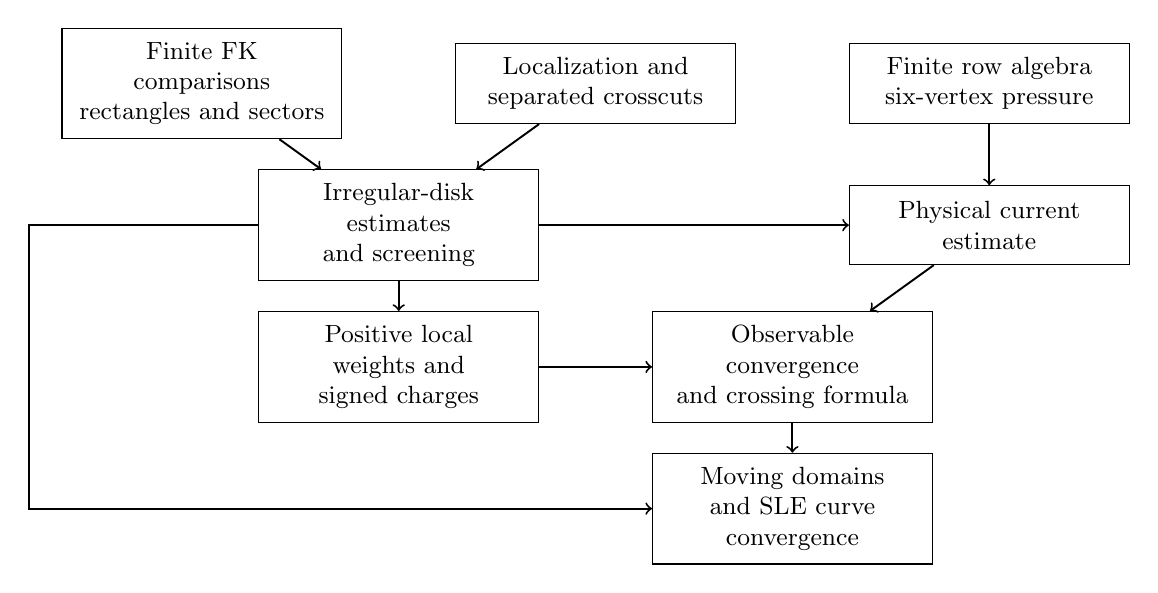
\begin{tikzpicture}[x=1cm,y=1cm,font=\small,
  block/.style={draw,align=center,text width=3.2cm,minimum height=1cm,inner sep=5pt},
  flow/.style={->,line width=.7pt}]
  \node[block] (finite) at (0,0) {Finite FK comparisons\\rectangles and sectors};
  \node[block] (local) at (5,0)
    {Localization and\\separated crosscuts};
  \node[block] (rows) at (10,0) {Finite row algebra\\six-vertex pressure};
  \node[block] (disks) at (2.5,-1.8) {Irregular-disk estimates\\and screening};
  \node[block] (current) at (10,-1.8) {Physical current\\estimate};
  \node[block] (charges) at (2.5,-3.6) {Positive local\\weights and\\signed charges};
  \node[block] (observable) at (7.5,-3.6) {Observable convergence\\and crossing formula};
  \node[block] (sle) at (7.5,-5.4) {Moving domains\\and SLE curve\\convergence};
  \draw[flow] (finite) -- (disks);
  \draw[flow] (local) -- (disks);
  \draw[flow] (rows) -- (current);
  \draw[flow] (disks) -- (current);
  \draw[flow] (disks) -- (charges);
  \draw[flow] (charges) -- (observable);
  \draw[flow] (current) -- (observable);
  \draw[flow] (observable) -- (sle);
  \draw[flow] (disks.west) -- (-2.2,-1.8) -- (-2.2,-5.4) -- (sle.west);
\end{tikzpicture}
\caption{The main proof dependencies. Localization in split tiled disks supplies the clear approaches and separated cuts needed to pass from finite network comparisons to actual-path decay. The disk estimates then feed both the local weight comparisons and the plane interpretation of the current. They also enter the moving-domain argument directly, through crossing estimates uniform over stopped exploration histories.}
\label{fig:dependencies}
\end{figure}


Appendix~\ref{sec:finite-calculus} gives the finite current identities,
extraction formulas, and reflection statements used by the observable.
Its norm consequence additionally uses the physical current estimate.
